%% ΠΕΡΙΓΡΑΦΗ ΠΕΡΙΠΤΩΣΕΩΝ ΧΡΗΣΗΣ
%% Σε αυτό το κεφάλαιο γίνεται αναλυτική περιγραφή των περιπτώσεων χρήσης
%% του συστήματος κρατήσεων ραντεβου (βασική και εναλλακτικές ροές).

\chapter{Περιπτώσεις Χρήσης}
Σε αυτό το κεφάλαιο θα γίνει η αναλυτική περιγραφή των περιπτώσεων χρήσης του συστήματος που υλοποιήθηκε. Θα περιγραφούν τόσο η βασική ροή όσο και οι εναλλακτικές ροές για όλες τις περιπτώσεις χρήσης. Το κεφάλαιο χωρίζεται σε τμήματα ανάλογα με τον ρόλο (actor) της εφαρμογής στον οποίο ανήκουν.

\section{Πελάτης}
\subsection{Κράτηση ραντεβού}
Η βασικότερη περίπτωση χρήσης της εφαρμογής είναι η διαδικασία της κράτησης ραντεβού του πελάτη με έναν πάροχο υπηρεσίας για την υπηρεσία που τον ενδιαφέρει. Πρόκειται για την κυριότερη περίπτωση χρήσης, μιας και το σύστημα έχει ως στόχο την ευκολότερη διαχείριση των ραντεβού με τους πελάτες. 

\textbf{ΒΑΣΙΚΗ ΡΟΗ}

Ο χρήστης μπαίνει στην σελίδα κράτησης ραντεβού και επιλέγει την υπηρεσία και τον πάροχο που τον ενδιαφέρει. Στην συνέχεια θα χρειαστεί να επιλέξει μια από τις διαθέσιμες ημερομηνίες και ώρες για να κλείσει το ραντεβού του. Αφού γίνει και αυτό θα πρέπει να συμπληρώσει τα στοιχεία του στην φόρμα που θα εμφανιστεί έτσι ώστε να μπορέσει η εταιρεία να έρθει σε επαφή μαζί του αν χρειαστεί. Τέλος ένα email θα σταλθεί πίσω στον πελάτη ότι το ραντεβού του έχει καταχωρηθεί με επιτυχία. Σε αυτό το email θα εμπεριέχεται και ένα link το οποίο θα του επιτρέπει να κάνει τροποποιήσει ή και να ακυρώσει το συγκεκριμένο ραντεβού.

\textbf{ΕΝΑΛΛΑΚΤΙΚΕΣ ΡΟΕΣ}

\begin{itemize}
\item Αν ο πελάτης αργήσει να επιλέξει ημερομηνία και στο ενδιάμεσο τον προλάβει ένας άλλος θα πρέπει να επιστραφεί μήνυμα το οποίο θα τον προτρέψει να βρει άλλη ημερομηνία και ώρα για το ραντεβού του.
\item Όταν ο πελάτης συμπληρώσει τα στοιχεία του και αφήσει κενό ένα πεδίο το οποίο είναι υποχρεωτικό για να ολοκληρωθεί η διαδικασία, θα εμφανιστεί μήνυμα το οποίο θα τον προτρέψει να συμπληρώσει όλα τα υποχρεωτικά πεδία.
\end{itemize}

\begin{figure}[ht!]
\centering
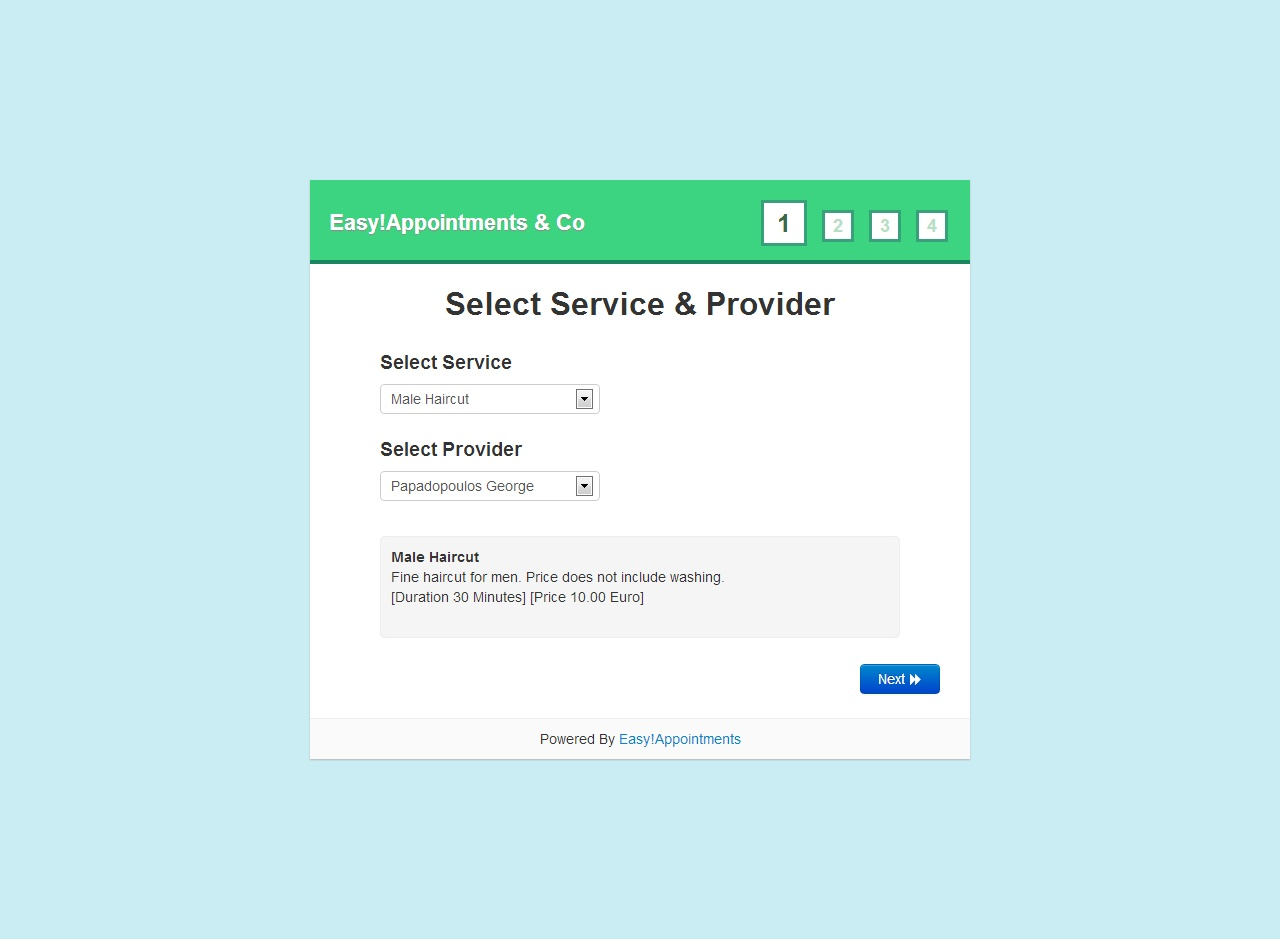
\includegraphics[width=130mm]{images/book-appointment.jpg}
\caption{Σελίδα κράτησης ραντεβού.}
\label{book-appointment}
\end{figure}

\begin{figure}[ht!]
\centering
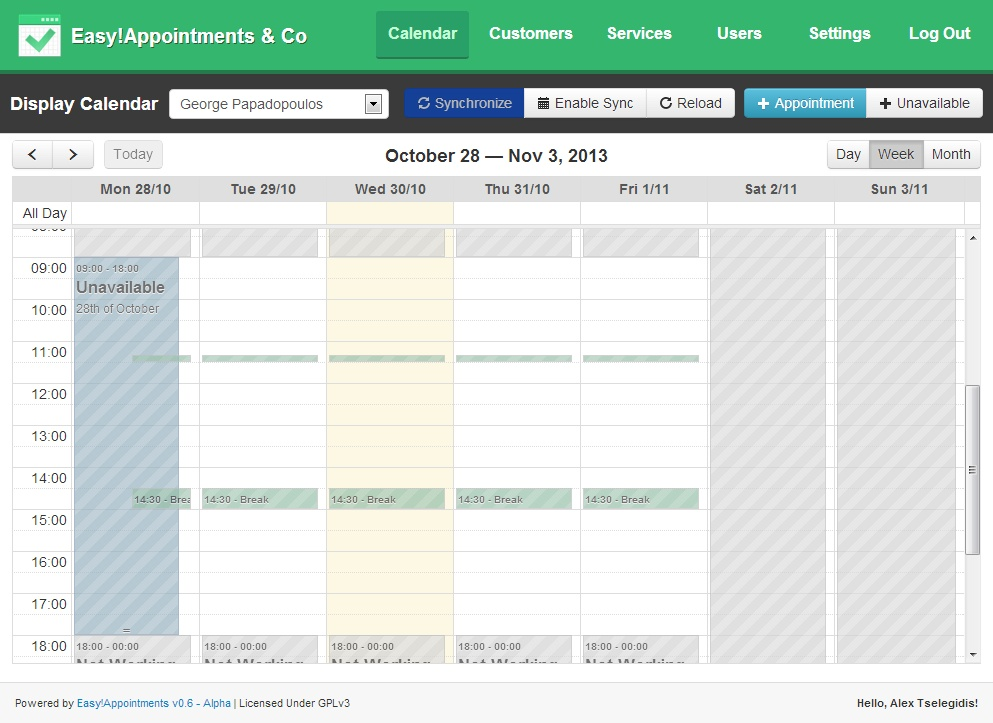
\includegraphics[width=130mm]{images/backend-calendar.jpg}
\caption{Σελίδα διαχείρισης ραντεβού.}
\label{backend-calendar}
\end{figure}

\begin{figure}[ht!]
\centering
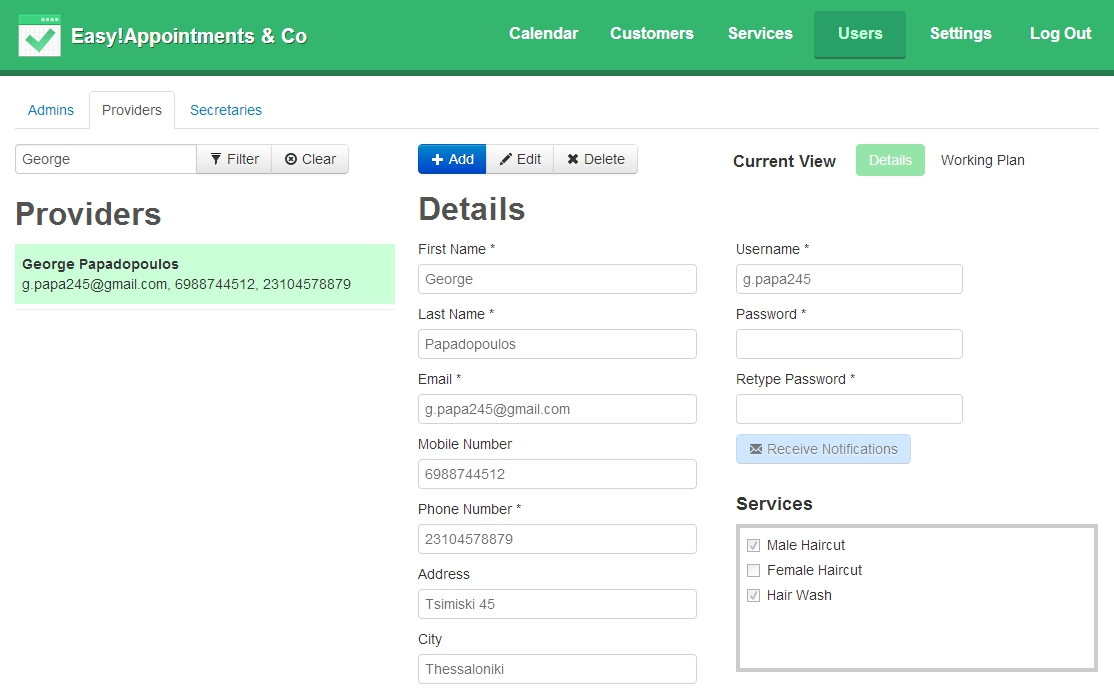
\includegraphics[width=130mm]{images/backend-providers.jpg}
\caption{Σελίδα διαχείρισης πάροχων υπηρεσιών.}
\label{backend-providers}
\end{figure}

\begin{figure}[ht!]
\centering
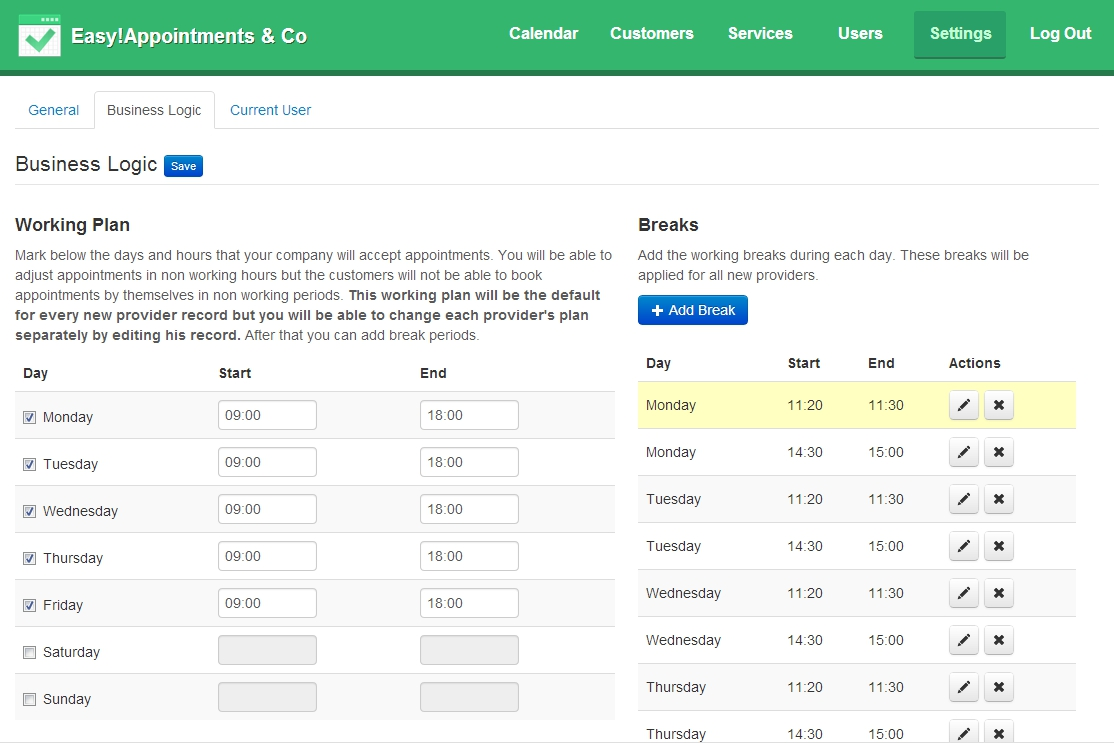
\includegraphics[width=130mm]{images/backend-settings.jpg}
\caption{Σελίδα ρυθμίσεων συστήματος.}
\label{book-settings}
\end{figure}

\subsection{Επεξεργασία - ακύρωση ραντεβού}
Εφόσον καταχωρηθεί ένα ραντεβού είναι πολύ σημαντικό να μπορέσει και να τροποποιηθεί με κάποιον τρόπο. Το σύστημα από την στιγμή που καταχωρεί ένα ραντεβού κρατάει και τα στοιχεία του πελάτη σε μια εγγραφή. Παρ' όλα αυτά δεν θα ήταν καλό να αναγκάζει τον πελάτη να δημιουργεί νέο χρήστη (με username και password) έτσι ώστε να μπορέσει να κάνει αλλαγές. Κάτι τέτοιο θα μείωνε την αποδοτικότητα της εφαρμογής μιας και προσθέτει ένα επιπλέον βήμα στην όλη διαδικασία, το οποίο μάλιστα θεωρείται εκνευριστικό αφού ένας μέσος χρήστης του διαδικτύου θα χρειαστεί να δημιουργήσει δεκάδες λογαριασμούς σε διάφορες ιστοσελίδες. Λαμβάνοντας αυτά υπόψιν για να μπορέσει ο πελάτης να πραγματοποιήσει αλλαγές ή και ακύρωση σε κάποιο ραντεβού του θα ακολουθεί έναν μοναδικό σύνδεσμο ο οποίος θα του έρχεται με email.

\textbf{ΒΑΣΙΚΗ ΡΟΗ}

Ο χρήστης ολοκληρώνει την διαδικασία κράτησης ραντεβού. Σε αυτήν την διαδικασία έχει ήδη δώσει το email του στο οποίο στέλνεται ένα email με τις πληροφορίες του ραντεβού που έχει κάνει κράτηση και μαζί έναν σύνδεσμο ο οποίος επιτρέπει στον χρήστη να πραγματοποιήσει αλλαγές στο συγκεκριμένο ραντεβού ή και να το ακυρώσει. Αφού ο χρήστης ακολουθήσει τον σύνδεσμο θα βρεθεί σε μια σελίδα η οποία θα περιέχει τις πληροφορίες του ραντεβού και θα του επιτρέπει να πραγματοποιήσει αλλαγές. Όταν ολοκληρώσει την διαδικασία θα πατάει ένα κουμπί το οποίο θα αποθηκεύει τις αλλαγές και ένα νέο email θα έρχεται πάλι στον χρήστη αλλά και στον συγκεκριμένο πάροχο ότι έχουν πραγματοποιηθεί αλλαγές στο πλάνο του.

\textbf{ΕΝΑΛΛΑΚΤΙΚΕΣ ΡΟΕΣ}

\begin{itemize}
\item Ο χρήστης μπορεί εν τέλη να μην θέλει να αποθηκεύσει τις αλλαγές του και έτσι να κλείσει την σελίδα.
\item Ο διαχειριστής του συστήματος μπορεί να έχει ορίσει ένα χρονικό περιθώριο πριν το ραντεβού, στο οποίο δεν επιτρέπεται να γίνονται αλλαγές (λόγω σταθερότητας του πλάνου). Αν ο χρήστης βρίσκεται μέσα σε αυτό το περιθώριο τότε θα εμφανιστεί μήνυμα το οποίο θα τον ενημερώνει για τον λόγο τον οποίο δεν μπορεί να πραγματοποιήσει αλλαγές στο ραντεβού του. 
\end{itemize}

\section {Πάροχος Υπηρεσιών}
\subsection {Συγχρονισμός πλάνου με το Google Calendar}
Βασικό στοιχείο για την χρησιμότητα και την απόδοση του συστήματος είναι η διαχείριση των δεδομένων να γίνεται από πολλά συστήματα. Κάτι τέτοιο μπορεί να επιτευχθεί με τον συγχρονισμό των ραντεβού με το Google Calendar API. Σε αυτό ο χρήστης θα μπορεί να πραγματοποιεί αλλαγές στο πλάνο του μέσω του Google Calendar και αυτές να εφαρμόζονται και στο σύστημα κρατήσεων ραντεβού κάνοντας έτσι την εργασία του πολύ εύκολη.

\textbf{ΒΑΣΙΚΗ ΡΟΗ}

Ο χρήστης βλέπει το πλάνο του μέσω της υπηρεσίας Google Calendar και προσθέτει ένα συμβάν κατά την διάρκεια του οποίο δεν είναι διαθέσιμος. Έπειτα από λίγο τρέχει χειροκίνητα τον συγχρονισμό από το Easy!Appointments και αυτό ανακαλύπτει ότι υπάρχει ένα νέο συμβάν στο Google Calendar το οποίο δεν είναι καταχωρημένο στην βάση δεδομένων του. Αμέσως μετά παίρνει τα στοιχεία του νέου συμβάντος μέσω του API που παρέχει η Google και το αποθηκεύει στην βάση δεδομένων έτσι ώστε να μην είναι διαθέσιμος ο πάροχος την συγκεκριμένη χρονική στιγμή. Την επόμενη φορά που θα πάει ένας πελάτης να κλείσει ραντεβού με τον συγκεκριμένο πάροχο θα δει ότι το συγκεκριμένο χρονικό διάστημα δεν είναι διαθέσιμο.

\textbf{ΕΝΑΛΛΑΚΤΙΚΕΣ ΡΟΕΣ}

\begin{itemize}
\item Πιθανό είναι να γίνει μια αλλαγή σε ένα συγχρονισμένο συμβάν στο Google Calendar το οποίο όμως να έχει αλλαχθεί και στο Easy!Appointments. Σε αυτήν την περίπτωση θεωρείται ότι υπερισχύει η αλλαγή που έχει γίνει στο Easy!Appointments διότι δεν υπάρχει η δυνατότητα να ελεγχθεί και στα δύο συστήματα το ποια χρονική στιγμή έχει γίνει η τροποποίηση.
\end{itemize}

\subsection {Διαχείριση ραντεβού}
Όπως και ο πελάτης, έτσι και ο πάροχος υπηρεσιών θα πρέπει να έχει την δυνατότητα να διαχειρίζεται τα ραντεβού του. Με αυτόν τον τρόπο θα έχει την δυνατότητα να πραγματοποιεί αλλαγές στο ημερολόγιο του, να αλλάζει την ημερομηνία των ραντεβού του και να καθορίζει το πλάνο του καταπώς τον βολεύει. Το Easy!Appointments εμφανίζει όλα τα ραντεβού σε ημερολόγιο, στο οποίο ο χρήστης μπορεί να περιηγηθεί χρονικά.

\textbf{ΒΑΣΙΚΗ ΡΟΗ}

Ο χρήστης ενημερώνεται από τον προϊστάμενο του ότι θα πρέπει να πραγματοποιήσει κάποια εργασία σε ένα χρονικό διάστημα στο οποίο υπάρχουν καταχωρημένα ραντεβού με πελάτες της εταιρείας. Κάποια από τα ραντεβού μπορεί να τα αναλάβει κάποιος άλλος πάροχος και για αυτόν τον λόγο ο χρήστης επεξεργάζεται αυτά τα ραντεβού και αλλάζει τον πάροχο τους έτσι ώστε να μετατεθούν στο πλάνου του αντίστοιχου χρήστη. Όσα περισσέψουν θα χρειαστεί να τα μεταφέρει χρονικά ή να τα διαγράψει προτείνοντας στους πελάτες να κλείσουν κάποια άλλη στιγμή.

\textbf{ΕΝΑΛΛΑΚΤΙΚΕΣ ΡΟΕΣ}

\begin{itemize}
\item Καθώς ο πάροχος υπηρεσιών επεξεργάζεται ένα ραντεβού μπορεί να αποφασίσει ότι δεν θέλει να αποθηκεύσει τις αλλαγές που έχει κάνει και έτσι πατάει το κουμπί ακύρωσης αποτρέποντας την ενημέρωση των δεδομένων στην βάση.
\item Σε αντίθεση με τον πελάτη, ένας πάροχος υπηρεσιών μπορεί να αλλάξει την διάρκεια ενός ραντεβού ανεξάρτητα από το πόση ώρα διαρκεί η υπηρεσία που θα παρέχει. Οπότε στην φόρμα επεξεργασίας ενός ραντεβού υπάρχει η δυνατότητα επιλογής ημερομηνίας και ώρας έναρξης και τερματισμού του ραντεβού.
\end{itemize}

\subsection{Λήψη ειδοποιήσεων από το σύστημα}
Κάθε φορά που πραγματοποιείται μια ενέργεια που αφορά κάποιο ραντεβού στο σύστημα ο πάροχος υπηρεσίας θα ενημερώνεται με email (εκτός και αν απενεργοποιήσει αυτήν την ρύθμιση). Έτσι θα είναι πάντα ενήμερος σχετικά με την κατάσταση των ραντεβού του. Σε αυτά τα μηνύματα θα περιέχεται και ένα μοναδικό link το οποίο θα δίνει την δυνατότητα στον πάροχο να πραγματοποιήσει αλλαγές γρήγορα στο ραντεβού που τον ενδιαφέρει.

\textbf{ΒΑΣΙΚΗ ΡΟΗ}

Ο πάροχος υπηρεσιών μπαίνει στο σύστημα και πραγματοποιεί αλλαγές σε ένα ήδη καταχωρημένο ραντεβού. Με την αποθήκευση των αλλαγών αυτός και ο πελάτης θα λάβουν ένα email στο οποίο θα φαίνονται τα νέα στοιχεία του ραντεβού. Με αυτόν τον τρόπο μπορεί να επαληθευθεί ότι οι αλλαγές που έγιναν είναι σωστές και επίσης δίνεται η δυνατότητα στον χρήστη να χρησιμοποιήσει το link του ραντεβού για να πραγματοποιήσει άλλες αλλαγές, αν αυτό είναι απαραίτητο.

\subsection {Διαχείριση Πελατών}
Από την στιγμή που ένας πάροχος θα έχει το δικαίωμα να επεξεργαστεί τις πληροφορίες ενός ραντεβού θα μπορεί να επεξεργάζεται και τα στοιχεία των πελατών που υπάγονται σε αυτό. Με αυτήν την δυνατότητα θα μπορεί να είναι σε θέση να ενημερώσει κάποια πεδία στην εγγραφή του πελάτη τα οποία είναι πιθανώς λανθασμένα ή και να προσθέσει νέες πληροφορίες.

\textbf{ΒΑΣΙΚΗ ΡΟΗ}

Ο πάροχος μπαίνει στο σύστημα και επιλέγει να επεξεργαστεί κάποιο ραντεβού. Στην οθόνη επεξεργασίας του ραντεβού θα μπορέσει να τροποποιήσει και τα στοιχεία των πελατών. Όταν είναι έτοιμος μπορεί να αποθηκεύσει τις αλλαγές στην βάση δεδομένων.

\textbf{ΕΝΑΛΛΑΚΤΙΚΕΣ ΡΟΕΣ}

Ο πάροχος μπορεί να αλλάξει τα στοιχεία ενός πελάτη χωρίς να πραγματοποιήσει αλλαγές στις πληροφορίες του ραντεβού του ίδιου.

\section{Γραμματέας}
\subsection{Διαχείριση ραντεβού}
Ο χρήστης γραμματέας μπορεί να πραγματοποιήσει αλλαγές στα ραντεβού ενός ή περισσοτέρων πάροχων υπηρεσίας. Με αυτόν τον τρόπο μια εταιρεία μπορεί να αναθέσει όλη την διαχείριση των ραντεβού σε ένα άτομο και οι πάροχοι απλώς να βλέπουν τα ραντεβού τους στο πλάνο.

\textbf{ΒΑΣΙΚΗ ΡΟΗ}

Ο χρήστης γραμματέας δέχεται τηλεφώνημα από κάποιον πελάτη ο οποίος επιθυμεί να αλλάξει την ώρα του ραντεβού του αλλά δεν έχει σύνδεση με το διαδίκτυο στο σημείο που βρίσκεται. Έτσι ο γραμματέας πραγματοποιεί την αλλαγή του ραντεβού καταπώς μπορεί να βολεύει τόσο τον πάροχο υπηρεσίας όσο και τον πελάτη. Όταν τελειώσει μπορεί να αποθηκεύσει τις αλλαγές στο σύστημα.

\subsection{Διαχείριση πελατών}
Εκτός των ραντεβού, ο χρήστης γραμματέας είναι σε θέση να πραγματοποιήσει αλλαγές και στα στοιχεία των πελατών οργανώνοντας και κρατώντας πλήρη πελατολόγιο για την επιχείριση. Μελλοντικά θα είναι σε θέση να βρίσκει πολύ εύκολα οποιονδήποτε πελάτη της επιχείρισης και να βλέπει τα στοιχεία του.

\textbf{ΒΑΣΙΚΗ ΡΟΗ}

Ο γραμματέας πηγαίνει στο backend στην σελίδα τον πελατών και φιλτράρει τον πελάτη που τον ενδιαφέρει και αμέσως βλέπει τα στοιχεία του. Πολύ εύκολα μπορεί να πραγματοποιήσει αλλαγές αλλά και να τον διαγράψει από το σύστημα. 

\textbf{ΕΝΑΛΛΑΚΤΙΚΕΣ ΡΟΕΣ}

\begin{itemize}
\item Ο γραμματέας μπορεί να επεξεργαστεί τα στοιχεία ενός πελάτη και την στιγμή που επεξεργάζεται ένα ραντεβού. Παρόλα αυτά σε αυτήν την περίπτωση κυρίαρχη οντότητα είναι το ραντεβού και έτσι ο χρήστης δεν έχει την δυνατότητα να φιλτράρει τους πελάτες καταπώς θέλει. Επίσης ένας πελάτης μπορεί να διαγραφεί μόνο όταν διαγραφεί και το ραντεβού του.
\end{itemize}

\section{Διαχειριστής}
\subsection{Εγκατάσταση της εφαρμογής}
Αυτή η περίπτωση χρήσης περιλαμβάνει την ρύθμιση του server όπου θα τρέξει το Easy!Appointments και την δημιουργία του λογαριασμού του διαχειριστή. Επίσης μπορεί να καθοριστούν και τα κλειδιά που απαιτούνται για την χρήση του Google Calendar API.

\textbf{ΒΑΣΙΚΗ ΡΟΗ} 

Ο διαχειριστής τοποθετεί τα αρχεία της εφαρμογής στον server του και πηγαίνει με τον περιηγητή στην διεύθυνση που δείχνει τον κύριο κατάλογο. Η εφαρμογή καταλαβαίνει ότι δεν έχει ακόμα πραγματοποιηθεί εγκατάσταση και μεταφέρει τον χρήστη στην διαδικασία εγκατάστασης. Σε αυτήν την διαδικασία ο διαχειριστής θα πρέπει να ορίσει σημαντικά στοιχεία που αφορούν την λειτουργία του συστήματος και τα στοιχεία του λογαριασμού του. Όλα αυτά τα στοιχεία βέβαια θα είναι διαθέσιμα προς επεξεργασία από την αντίστοιχη σελίδα στο backend.

\subsection{Παραμετροποίηση της εφαρμογής}
Για να μπορέσει να λειτουργήσει η εφαρμογή σύμφωνα με την μορφή της επιχείρησης θα χρειαστεί να παραμετροποιηθεί από τον διαχειριστή. Η παραμετροποίηση περιλαμβάνει τα ωράρια λειτουργίας της επιχείρησης, την διαχείριση των υπηρεσιών που θα είναι διαθέσιμες προς το κοινό καθώς και την διαχείριση των πάροχων υπηρεσιών.

\textbf{ΒΑΣΙΚΗ ΡΟΗ}

Ο διαχειριστής εισέρχεται στο backend μέρος της εφαρμογής και επιλέγει την σελίδα των ρυθμίσεων. Εκεί έχει την δυνατότητα να θέσει τις τιμές σε διάφορες παραμέτρους οι οποίες καθορίζουν τον τρόπο με τον οποίο λειτουργεί το σύστημα. Στόχος είναι αυτός να συμβαδίζει με τον τρόπο λειτουργίας της επιχείρισης έτσι ώστε να μπορεί η εταιρεία να επωφεληθεί από το Easy!Appointments.

\subsection{Διαχείριση ραντεβού}
Ο διαχειριστής ως χρήστης έχει πρόσβαση σε όλες τις πληροφορίες του συστήματος. Έτσι μπορεί να μεταβάλει και να προσθέσει ραντεβού στο σύστημα σαν να ήταν ένας πάροχος υπηρεσιών ή ένας χρήστης γραμματέας.

\textbf {ΒΑΣΙΚΗ ΡΟΗ}

Ο διαχειριστής συνδέεται στο backend μέρος της εφαρμογής και πηγαίνει στην σελίδα του ημερολογίου. Εκεί μπορεί να δει τα ραντεβού όλων των πάροχων υπηρεσιών και να πραγματοποιήσει αλλαγές σε αυτά. Με το που αποθηκευτούν οι αλλαγές σε ένα ραντεβού ο πελάτης και ο πάροχος θα ενημερωθούν με email, όπως θα γινόταν δηλαδή αν την επεξεργασία την έκανε ένας πάροχος.

\subsection {Διαχείριση χρηστών}
Τις υπηρεσίες που προσφέρει η εταιρεία τις αναλαμβάνουν κάποιοι υπάλληλοι (ή ομάδες υπαλλήλων), οι οποίοι αναφέρονται στο σύστημα ως πάροχοι υπηρεσιών. Τα στοιχεία τους και τις αρμοδιότητές τους μέσα στο σύστημα τα ορίζει μόνο ο διαχειριστής του συστήματος, από το backend μέρος της εφαρμογής. Επίσης είναι δυνατή η διαχείριση των διαχειριστών, γραμματειών και πελατών του συστήματος.

\textbf{ΒΑΣΙΚΗ ΡΟΗ}

Ο διαχειριστής της εφαρμογής συνδέεται στο backend και πηγαίνει στην σελίδα των πάροχων υπηρεσίας. Εκεί βλέπει μια λίστα με τους ήδη καταχωρημένους πάροχους. Αν θέλει μπορεί να προσθέσει έναν καινούργιο χρήστη ή να επεξεργαστεί και να διαγράψει κάποια εγγραφή που υπάρχει ήδη στην βάση δεδομένων.

\subsection {Διαχείριση υπηρεσιών}
Οι πελάτες που θα επισκέπτονται τον ιστότοπο του Easy!Appointments της επιχείρησης θα κλείνουν ραντεβού για συγκεκριμένες υπηρεσίες. Το ποιες υπηρεσίες θα είναι διαθέσιμες και ποιοι πάροχοι υπηρεσιών μπορούν να εξυπηρετήσουν τι, το διαχειρίζεται ο διαχειριστής του συστήματος. Αποτελεί υποπερίπτωση χρήσης της παραμετροποίησης της εφαρμογής.